\documentclass[11pt,a4paper,twoside]{book}

% Package imports
\usepackage[utf8]{inputenc}
\usepackage[T1]{fontenc}
\usepackage{geometry}
\usepackage{xcolor}
\usepackage{graphicx}
\usepackage{fancyhdr}
\usepackage{titlesec}
\usepackage{tcolorbox}
\usepackage{tikz}
\usepackage{pgfplots}
\usepackage{booktabs}
\usepackage{hyperref}
\usepackage{listings}
\usepackage{amsmath}
\usepackage{amssymb}
\usepackage{enumitem}
\usepackage{caption}
\usepackage{float}

\usetikzlibrary{shapes,arrows,positioning,shadows,calc}
\pgfplotsset{compat=1.18}

% Page geometry
\geometry{
    top=2.5cm,
    bottom=3cm,
    left=2.5cm,
    right=2.5cm,
    footskip=1.5cm
}

% NVIDIA Color Definitions
\definecolor{nvidiagreen}{HTML}{76B900}
\definecolor{nvidiadark}{HTML}{000000}
\definecolor{nvidiagray}{HTML}{333333}
\definecolor{nvidialightgray}{HTML}{CCCCCC}
\definecolor{nvidiawhite}{HTML}{FFFFFF}

% Hyperref setup
\hypersetup{
    colorlinks=true,
    linkcolor=nvidiagreen,
    urlcolor=nvidiagreen,
    citecolor=nvidiagreen,
    pdfborder={0 0 0}
}

% Title formatting
\titleformat{\chapter}[display]
{\normalfont\huge\bfseries\color{nvidiagreen}}
{\chaptertitlename\ \thechapter}{20pt}{\Huge\color{nvidiagreen}}

\titleformat{\section}
{\normalfont\Large\bfseries\color{nvidiagreen}}
{\thesection}{1em}{}

\titleformat{\subsection}
{\normalfont\large\bfseries\color{nvidiagreen}}
{\thesubsection}{1em}{}

% Custom header and footer
\fancypagestyle{mainpagestyle}{
    \fancyhf{}
    \fancyhead[LE,RO]{\color{nvidiagreen}\thepage}
    \fancyhead[LO]{\color{nvidiagray}\nouppercase{\rightmark}}
    \fancyhead[RE]{\color{nvidiagray}\nouppercase{\leftmark}}
    
    % Custom footer with three columns
    \fancyfoot[L]{\small\color{nvidiagray}\href{https://easy-ai-labs.lovable.app/}{Easy AI Labs}}
    \fancyfoot[C]{\small\color{nvidiagray}\href{https://www.linkedin.com/in/yashkavaiya}{Yash Kavaiya}}
    \fancyfoot[R]{\small\color{nvidiagray}\href{https://www.linkedin.com/company/genai-guru}{Gen AI Guru}}
    
    \renewcommand{\headrulewidth}{0.5pt}
    \renewcommand{\footrulewidth}{0.5pt}
    \renewcommand{\headrule}{\hbox to\headwidth{\color{nvidiagreen}\leaders\hrule height \headrulewidth\hfill}}
    \renewcommand{\footrule}{\hbox to\headwidth{\color{nvidiagreen}\leaders\hrule height \footrulewidth\hfill}}
}

\pagestyle{mainpagestyle}

% Code listing style
\lstdefinestyle{cudastyle}{
    language=C++,
    backgroundcolor=\color{nvidiadark},
    commentstyle=\color{nvidialightgray},
    keywordstyle=\color{nvidiagreen}\bfseries,
    numberstyle=\tiny\color{nvidialightgray},
    stringstyle=\color{nvidiagreen},
    basicstyle=\ttfamily\small\color{nvidiawhite},
    breakatwhitespace=false,
    breaklines=true,
    captionpos=b,
    keepspaces=true,
    numbers=left,
    numbersep=5pt,
    showspaces=false,
    showstringspaces=false,
    showtabs=false,
    tabsize=4,
    frame=single,
    rulecolor=\color{nvidiagreen}
}

\lstset{style=cudastyle}

% Custom boxes
\newtcolorbox{nvidiabox}[1]{
    colback=nvidiadark,
    colframe=nvidiagreen,
    fonttitle=\bfseries\color{nvidiawhite},
    title=#1,
    arc=3mm,
    boxrule=2pt,
    coltext=nvidiawhite
}

\newtcolorbox{highlightbox}{
    colback=nvidiagreen!10,
    colframe=nvidiagreen,
    arc=2mm,
    boxrule=1pt
}

% Document information
\title{\Huge\bfseries\color{nvidiagreen} CUDA Programming Guide\\[0.5cm]
\Large Parallel Computing Platform}
\author{\Large Yash Kavaiya\\[0.2cm]
\normalsize Easy AI Labs \& Gen AI Guru}
\date{\today}

\begin{document}

% Title page
\begin{titlepage}
    \centering
    \vspace*{2cm}
    
    {\Huge\bfseries\color{nvidiagreen} CUDA Programming Guide\par}
    \vspace{0.5cm}
    {\Large\color{nvidiagray} Understanding Parallel Computing Platform\par}
    \vspace{2cm}
    
    
\begin{tikzpicture}
        \draw[nvidiagreen, line width=3pt] (0,0) -- (10,0);
        \draw[nvidiagreen, line width=2pt] (0,-0.3) -- (10,-0.3);
    \end{tikzpicture}
    
    \vspace{2cm}
    {\Large\bfseries Yash Kavaiya\par}
    \vspace{0.5cm}
    {\large Easy AI Labs \& Gen AI Guru\par}
    
    \vfill
    
    {\large \today\par}
\end{titlepage}

% Table of Contents
\tableofcontents
\clearpage

% Main Content
\chapter{Introduction to CUDA}

\section{What is CUDA?}

\begin{highlightbox}
\textbf{CUDA} stands for \textbf{Compute Unified Device Architecture}. It is a parallel computing platform and programming model developed by NVIDIA that enables dramatic increases in computing performance by harnessing the power of the Graphics Processing Unit (GPU).
\end{highlightbox}

CUDA is a revolutionary framework that allows developers to leverage the massive parallel processing power of NVIDIA GPUs for general-purpose computing tasks, not just graphics rendering.

\subsection{Key Features}

\begin{itemize}[itemsep=10pt]
    \item \textbf{Parallel Computing:} Execute thousands of threads simultaneously
    \item \textbf{General Purpose:} Use GPU for non-graphics computations
    \item \textbf{Language Support:} Write code in C, C++, Python, and more
    \item \textbf{High Performance:} Dramatically accelerate compute-intensive applications
\end{itemize}

\section{The Kitchen Analogy}

To understand CUDA's power, consider this analogy:

\begin{nvidiabox}{Traditional CPU Approach}
Imagine a small kitchen with a head chef and 2-3 skilled assistants. They can make complex dishes efficiently. However, when you receive an order for 100 servings of French fries, they must:
\begin{itemize}
    \item Chop potatoes one by one
    \item Fry them individually
    \item Pack them sequentially
\end{itemize}
This is time-consuming, even though French fries aren't complex to make.
\end{nvidiabox}

\vspace{1cm}

\begin{nvidiabox}{CUDA GPU Approach}
Now imagine the same kitchen, but with 100 trainee cooks available. While they may not be skilled at complex tasks, they excel at repetitive operations. With proper coordination:
\begin{itemize}
    \item 25 cooks chop potatoes simultaneously
    \item 25 cooks fry the potatoes in parallel
    \item 25 cooks handle seasoning
    \item 25 cooks pack the final product
\end{itemize}
The result? All 100 orders completed much faster!
\end{nvidiabox}

\subsection{The Language Barrier Problem}

\begin{figure}[H]
    \centering
    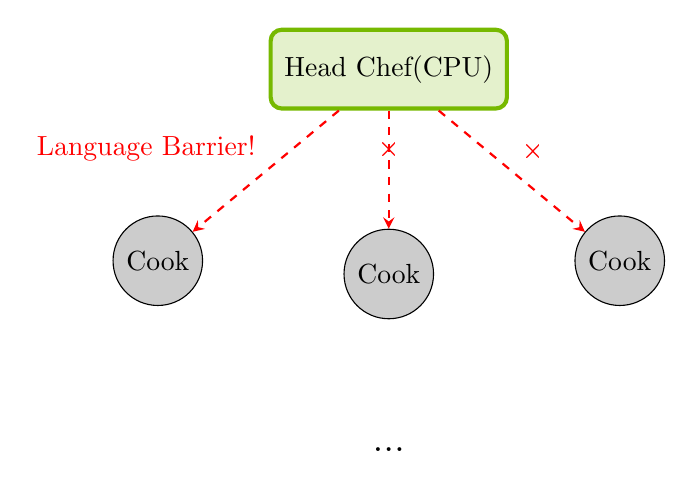
\begin{tikzpicture}[node distance=2cm]
        % Define styles
        \tikzstyle{chef} = [rectangle, rounded corners, minimum width=3cm, minimum height=1cm, text centered, draw=nvidiagreen, fill=nvidiagreen!20, line width=1.5pt]
        \tikzstyle{cook} = [circle, minimum width=1cm, text centered, draw=nvidiadark, fill=nvidialightgray]
        \tikzstyle{arrow} = [thick,->,>=stealth,color=red]
        
        % Chef
        \node (chef) [chef] {Head Chef\\(CPU)};
        
        % Cooks
        \node (cook1) [cook, below left=1.5cm and 1cm of chef] {Cook};
        \node (cook2) [cook, below=1.5cm of chef] {Cook};
        \node (cook3) [cook, below right=1.5cm and 1cm of chef] {Cook};
        \node (dots) [below=1.5cm of cook2] {\Large...};
        
        % Language barrier
        \draw[arrow, red, dashed] (chef) -- node[above left, text=red] {Language Barrier!} (cook1);
        \draw[arrow, red, dashed] (chef) -- node[above, text=red] {×} (cook2);
        \draw[arrow, red, dashed] (chef) -- node[above right, text=red] {×} (cook3);
        
    \end{tikzpicture}
    \caption{Communication problem without CUDA}
\end{figure}

\textbf{The Problem:} If the head chef speaks English but the trainee cooks speak a different language, there's a communication barrier. Despite having capable workers, they remain idle because they don't understand the instructions.

\textbf{The Solution:} CUDA acts as a translator, enabling the CPU (chef) to effectively communicate with the GPU cores (trainee cooks).

\chapter{Evolution of GPU Computing}

\section{Before CUDA: The Graphics-Only Era}

\begin{table}[H]
\centering
\caption{GPU Capabilities Before and After CUDA}
\begin{tabular}{@{}lll@{}}
\toprule
\textbf{Aspect} & \textbf{Before CUDA} & \textbf{After CUDA} \\ 
\midrule
\textbf{Primary Use} & Graphics rendering only & General-purpose computing \\
\textbf{Programming} & OpenGL, DirectX & C, C++, Python, Fortran \\
\textbf{Access Method} & Graphics API only & Direct GPU programming \\
\textbf{Non-graphics Work} & Required "tricks" & Native support \\
\textbf{Development} & Complex, impractical & Straightforward \\
\textbf{CPU Utilization} & Heavy lifting on CPU & Workload distribution \\
\textbf{GPU Core Usage} & Idle for compute & Fully utilized \\
\bottomrule
\end{tabular}
\end{table}

\subsection{The Graphics API Limitation}

Originally, GPUs were designed exclusively for rendering graphics. Developers could only communicate with GPUs through graphics APIs:

\begin{itemize}
    \item \textbf{OpenGL:} Open Graphics Library
    \item \textbf{DirectX:} Microsoft's graphics API
\end{itemize}

These APIs could send instructions for:
\begin{itemize}
    \item Rendering pixels
    \item Creating brightness effects
    \item Illumination calculations
    \item Texture mapping
\end{itemize}

\begin{highlightbox}
\textbf{The Problem:} General-purpose code written in C, C++, or Python could only run on the CPU. If you wanted to perform non-graphics work like physics simulations, financial modeling, or AI computations, you had to "trick" the GPU by disguising calculations as graphics operations.
\end{highlightbox}

\section{The CUDA Revolution}

\begin{figure}[H]
    \centering
    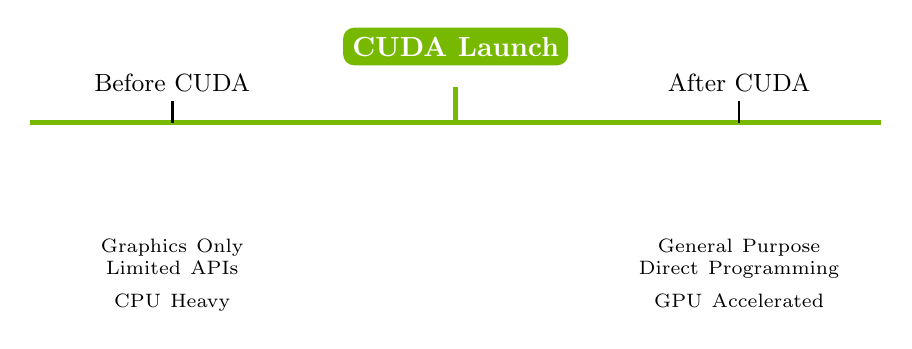
\begin{tikzpicture}[scale=0.9]
        % Timeline
        \draw[line width=2pt, nvidiagreen] (0,0) -- (12,0);
        
        % Before CUDA
        \draw[line width=1pt] (2,0) -- (2,0.3);
        \node[above] at (2,0.3) {\small Before CUDA};
        \node[below, text width=3cm, align=center] at (2,-1.5) {
            \scriptsize Graphics Only\\
            \scriptsize Limited APIs\\
            \scriptsize CPU Heavy
        };
        
        % CUDA Launch
        \draw[line width=2pt, nvidiagreen] (6,0) -- (6,0.5);
        \node[above, fill=nvidiagreen, text=white, rounded corners] at (6,0.8) {\textbf{CUDA Launch}};
        
        % After CUDA
        \draw[line width=1pt] (10,0) -- (10,0.3);
        \node[above] at (10,0.3) {\small After CUDA};
        \node[below, text width=3cm, align=center] at (10,-1.5) {
            \scriptsize General Purpose\\
            \scriptsize Direct Programming\\
            \scriptsize GPU Accelerated
        };
    \end{tikzpicture}
    \caption{The transformation brought by CUDA}
\end{figure}

\subsection{What CUDA Enables}

\begin{enumerate}[leftmargin=2cm, itemsep=8pt]
    \item \textbf{Direct GPU Programming:} Write native C, C++, or Python code that runs directly on the GPU
    \item \textbf{General-Purpose Acceleration:} Transform GPU from a graphics accelerator to a general-purpose computing powerhouse
    \item \textbf{Parallel Execution:} Harness thousands of GPU cores for simultaneous computation
    \item \textbf{Straightforward Development:} No more "tricking" the GPU—write parallel code naturally
\end{enumerate}

\chapter{CUDA Architecture}

\section{Software Stack}

\begin{figure}[H]
    \centering
    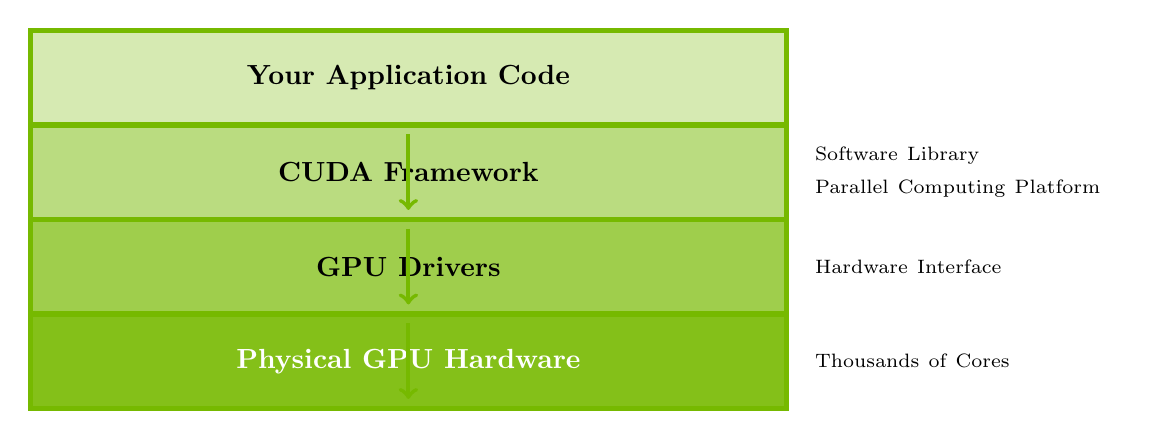
\begin{tikzpicture}[scale=1.2]
        % Application Layer
        \draw[fill=nvidiagreen!30, draw=nvidiagreen, line width=2pt] 
            (0,4) rectangle (8,5) node[pos=0.5] {\textbf{Your Application Code}};
        
        % CUDA Layer
        \draw[fill=nvidiagreen!50, draw=nvidiagreen, line width=2pt] 
            (0,3) rectangle (8,4) node[pos=0.5] {\textbf{CUDA Framework}};
        \node[right, text width=4cm] at (8.2,3.5) {\scriptsize Software Library\\
        \scriptsize Parallel Computing Platform};
        
        % Driver Layer
        \draw[fill=nvidiagreen!70, draw=nvidiagreen, line width=2pt] 
            (0,2) rectangle (8,3) node[pos=0.5] {\textbf{GPU Drivers}};
        \node[right, text width=4cm] at (8.2,2.5) {\scriptsize Hardware Interface};
        
        % Hardware Layer
        \draw[fill=nvidiagreen!90, draw=nvidiagreen, line width=2pt] 
            (0,1) rectangle (8,2) node[pos=0.5, text=white] {\textbf{Physical GPU Hardware}};
        \node[right, text width=4cm] at (8.2,1.5) {\scriptsize Thousands of Cores};
        
        % Arrows
        \foreach \y in {2,3,4} {
            \draw[->, line width=1.5pt, nvidiagreen] (4,\y-0.1) -- (4,\y-0.9);
        }
    \end{tikzpicture}
    \caption{CUDA software stack architecture}
\end{figure}

\section{Installation Steps}

To get started with CUDA, follow this installation sequence:

\begin{enumerate}[itemsep=12pt]
    \item \textbf{Install Physical GPU:} Ensure you have an NVIDIA GPU in your system
    \item \textbf{Install GPU Drivers:} Download and install the latest NVIDIA drivers for your GPU model
    \item \textbf{Install CUDA Toolkit:} Install the CUDA software library from NVIDIA's developer portal
    \item \textbf{Verify Installation:} Test the installation using sample programs
\end{enumerate}

\section{Programming Model}

\subsection{CPU vs GPU Execution}

\begin{table}[H]
\centering
\caption{CPU and GPU Roles in CUDA}
\begin{tabular}{@{}p{3cm}p{5cm}p{5cm}@{}}
\toprule
\textbf{Component} & \textbf{Role} & \textbf{Characteristics} \\ 
\midrule
\textbf{CPU (Host)} & Organizes and manages tasks & 
\begin{itemize}[leftmargin=*,nosep]
    \item Few powerful cores
    \item Complex control logic
    \item Sequential processing
    \item Task coordination
\end{itemize} \\[1cm]
\textbf{GPU (Device)} & Executes tasks in parallel & 
\begin{itemize}[leftmargin=*,nosep]
    \item Thousands of cores
    \item Simple control logic
    \item Massive parallelism
    \item Data processing
\end{itemize} \\
\bottomrule
\end{tabular}
\end{table}

\subsection{The Coordination Model}

Think of it like an orchestra:
\begin{itemize}
    \item \textbf{CPU = Conductor:} Gives instructions, manages timing, coordinates sections
    \item \textbf{GPU = Orchestra:} Hundreds of musicians playing their parts simultaneously
\end{itemize}

\chapter{CUDA Programming Concepts}

\section{Traditional vs Parallel Programming}

\begin{figure}[H]
    \centering
    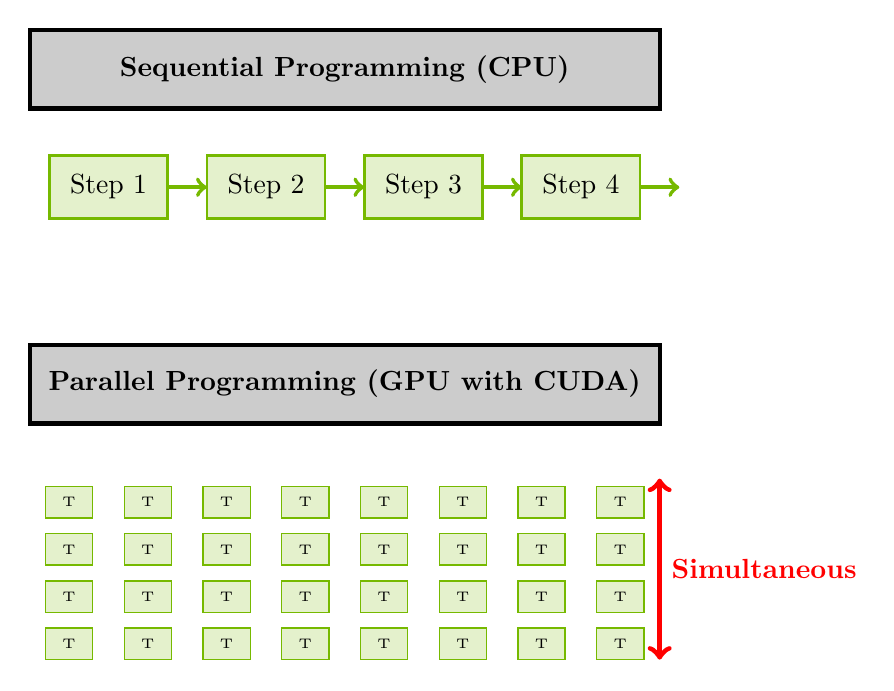
\begin{tikzpicture}
        % Traditional Sequential
        \node[draw=nvidiadark, fill=nvidialightgray, minimum width=8cm, minimum height=1cm, line width=1.5pt] at (0,3) (seq) {\textbf{Sequential Programming (CPU)}};
        
        \foreach \x/\label in {-3/Step 1, -1/Step 2, 1/Step 3, 3/Step 4} {
            \node[draw=nvidiagreen, fill=nvidiagreen!20, minimum width=1.5cm, minimum height=0.8cm, line width=1pt] at (\x,1.5) {\label};
            \draw[->, line width=1.5pt, nvidiagreen] (\x+0.75,1.5) -- (\x+1.25,1.5);
        }
        
        % Parallel Processing
        \node[draw=nvidiadark, fill=nvidialightgray, minimum width=8cm, minimum height=1cm, line width=1.5pt] at (0,-1) (par) {\textbf{Parallel Programming (GPU with CUDA)}};
        
        \foreach \y in {0,...,3} {
            \foreach \x in {-3.5,-2.5,-1.5,-0.5,0.5,1.5,2.5,3.5} {
                \node[draw=nvidiagreen, fill=nvidiagreen!20, minimum width=0.6cm, minimum height=0.4cm, line width=0.5pt] at (\x,-2.5-\y*0.6) {\tiny T};
            }
        }
        
        \draw[<->, line width=2pt, red] (4,-2.2) -- (4,-4.5) node[midway, right] {\textbf{Simultaneous}};
        
    \end{tikzpicture}
    \caption{Sequential vs Parallel execution models}
\end{figure}

\subsection{Programming Model Comparison}

\begin{nvidiabox}{Traditional Sequential Model}
\textbf{Approach:}
\begin{enumerate}
    \item Execute Step 1
    \item Wait for Step 1 to complete
    \item Execute Step 2
    \item Wait for Step 2 to complete
    \item Execute Step 3
    \item Continue...
\end{enumerate}
\textbf{Result:} Tasks completed one after another (serial execution)
\end{nvidiabox}

\vspace{0.5cm}

\begin{nvidiabox}{CUDA Parallel Model}
\textbf{Approach:}
\begin{enumerate}
    \item Break problem into smaller, identical tasks
    \item Launch thousands of threads (workers)
    \item All threads execute simultaneously
    \item Collect results when everyone finishes
\end{enumerate}
\textbf{Result:} Massive speedup through parallel execution
\end{nvidiabox}

\section{The Fence Painting Analogy}

\begin{figure}[H]
    \centering
    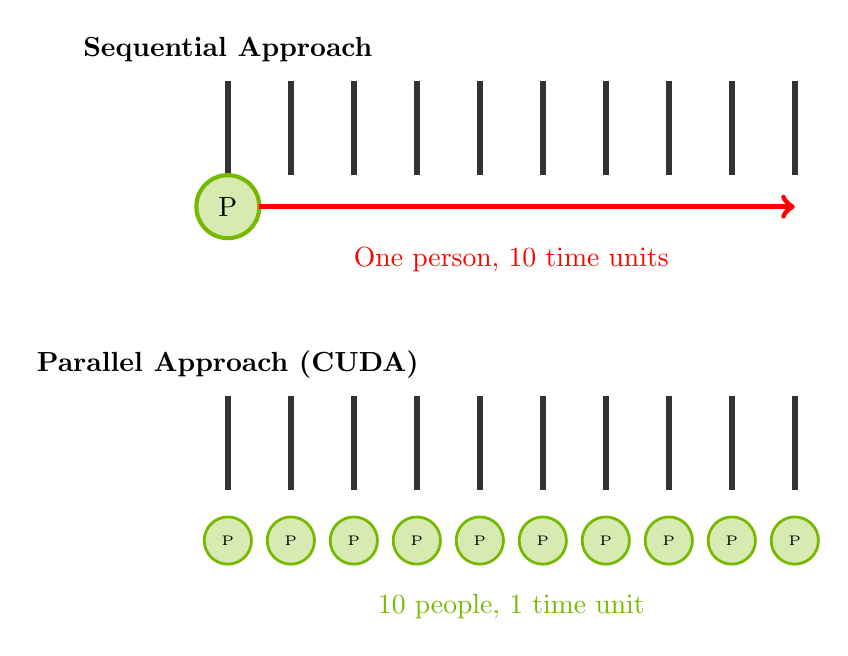
\begin{tikzpicture}[scale=0.8]
        % Sequential approach
        \node at (0,4) {\textbf{Sequential Approach}};
        \foreach \x in {0,...,9} {
            \draw[line width=2pt, nvidiagray] (\x,2) -- (\x,3.5);
        }
        \node[circle, draw=nvidiagreen, fill=nvidiagreen!30, minimum size=0.8cm, line width=1.5pt] at (0,1.5) {P};
        \draw[->, line width=2pt, red] (0.5,1.5) -- (9,1.5);
        \node[below, text=red] at (4.5,1) {One person, 10 time units};
        
        % Parallel approach
        \node at (0,-1) {\textbf{Parallel Approach (CUDA)}};
        \foreach \x in {0,...,9} {
            \draw[line width=2pt, nvidiagray] (\x,-3) -- (\x,-1.5);
            \node[circle, draw=nvidiagreen, fill=nvidiagreen!30, minimum size=0.6cm, line width=1pt] at (\x,-3.8) {\tiny P};
        }
        \node[below, text=nvidiagreen] at (4.5,-4.5) {10 people, 1 time unit};
        
    \end{tikzpicture}
    \caption{Fence painting: Sequential vs Parallel}
\end{figure}

Imagine painting a fence with multiple sections:

\textbf{Sequential Approach:}
\begin{itemize}
    \item One person paints section 1, then moves to section 2, then section 3...
    \item Total time: 10 sections × 1 time unit = 10 time units
\end{itemize}

\textbf{Parallel Approach with CUDA:}
\begin{itemize}
    \item 10 people each paint one section simultaneously
    \item Total time: 1 time unit (10× speedup!)
\end{itemize}

\section{CUDA's Role}

CUDA provides the tools to:
\begin{enumerate}[itemsep=10pt]
    \item \textbf{Organize} the thousand workers (GPU cores) effectively
    \item \textbf{Coordinate} their simultaneous execution
    \item \textbf{Distribute} tasks efficiently across all workers
    \item \textbf{Collect} and combine results from parallel execution
\end{enumerate}

\chapter{CUDA Applications}

\section{Application Domains}

CUDA enables GPU acceleration across numerous fields:

\begin{table}[H]
\centering
\caption{CUDA Application Domains}
\begin{tabular}{@{}llp{6cm}@{}}
\toprule
\textbf{Domain} & \textbf{Applications} & \textbf{Benefits} \\ 
\midrule
\textbf{AI/ML} & Deep Learning, Neural Networks & Training models 100× faster \\
\textbf{Scientific} & Physics simulations, Molecular dynamics & Complex calculations in parallel \\
\textbf{Finance} & Risk analysis, Options pricing & Real-time market analysis \\
\textbf{Medical} & CT/MRI reconstruction, Drug discovery & Faster diagnosis and research \\
\textbf{Video} & Encoding, Effects, Enhancement & Real-time video processing \\
\textbf{Graphics} & Ray tracing, 3D rendering & Photorealistic rendering \\
\bottomrule
\end{tabular}
\end{table}

\section{Performance Comparison}

\begin{figure}[H]
    \centering
    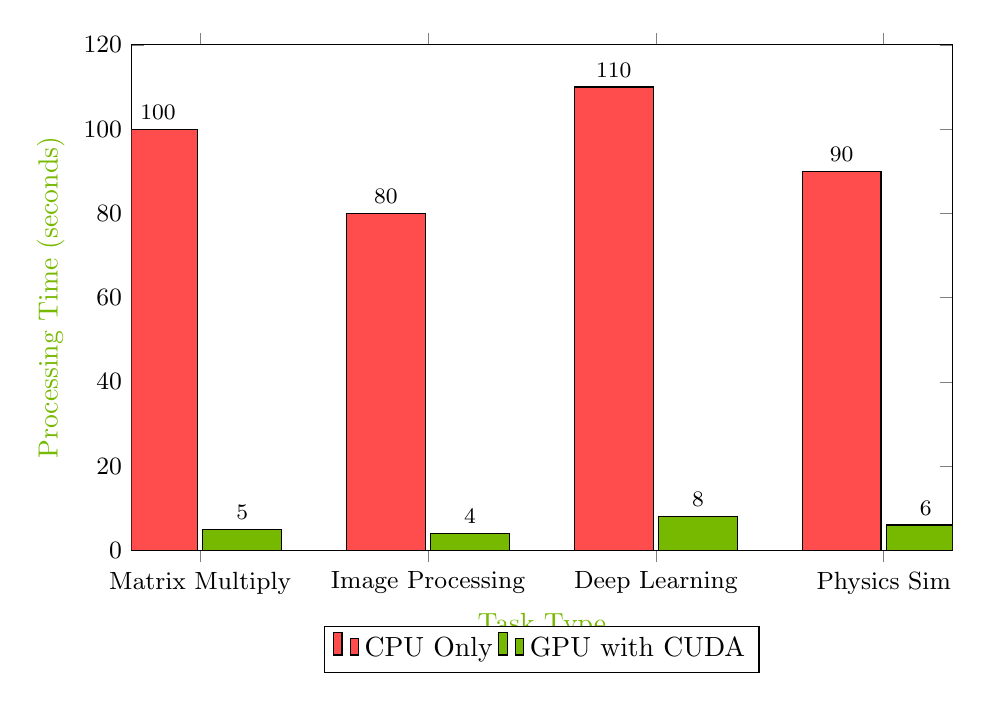
\begin{tikzpicture}
        \begin{axis}[
            ybar,
            bar width=1cm,
            width=12cm,
            height=8cm,
            ylabel={Processing Time (seconds)},
            xlabel={Task Type},
            symbolic x coords={Matrix Multiply, Image Processing, Deep Learning, Physics Sim},
            xtick=data,
            ymin=0,
            ymax=120,
            nodes near coords,
            legend style={at={(0.5,-0.15)}, anchor=north, legend columns=-1},
            ylabel style={color=nvidiagreen},
            xlabel style={color=nvidiagreen},
            tick label style={font=\small},
            every node near coord/.append style={font=\footnotesize}
        ]
        \addplot[fill=red!70] coordinates {(Matrix Multiply,100) (Image Processing,80) (Deep Learning,110) (Physics Sim,90)};
        \addplot[fill=nvidiagreen] coordinates {(Matrix Multiply,5) (Image Processing,4) (Deep Learning,8) (Physics Sim,6)};
        \legend{CPU Only, GPU with CUDA}
        \end{axis}
    \end{tikzpicture}
    \caption{CPU vs GPU performance comparison}
\end{figure}

\chapter{Understanding CUDA's Bridge}

\section{What CUDA Does}

\begin{highlightbox}
\Large\textbf{CUDA creates a bridge between normal programming code and GPU computing power.}
\end{highlightbox}

\subsection{Before CUDA}

\begin{itemize}[itemsep=10pt]
    \item \textbf{CPU:} Only component used for general computing
    \item \textbf{GPU:} Limited to graphics rendering
    \item \textbf{Limitations:}
    \begin{itemize}
        \item No image/video processing on GPU
        \item No 3D modeling computations
        \item No machine learning acceleration
        \item No scientific simulations
    \end{itemize}
\end{itemize}

\subsection{After CUDA}

\begin{itemize}[itemsep=10pt]
    \item \textbf{CPU:} Task coordination and management
    \item \textbf{GPU:} Parallel execution of compute-intensive tasks
    \item \textbf{Capabilities:}
    \begin{itemize}
        \item Full image and video processing
        \item Complex 3D modeling and simulation
        \item Accelerated machine learning and AI
        \item High-performance scientific computing
    \end{itemize}
\end{itemize}

\section{Language Support}

With CUDA, GPU workers understand regular programming languages:

\begin{lstlisting}[caption={Simple CUDA Kernel Example (C++)}, label={lst:cuda_example}]
__global__ void vectorAdd(float *a, float *b, float *c, int n) {
    // Get thread index
    int idx = blockIdx.x * blockDim.x + threadIdx.x;
    
    // Perform computation
    if (idx < n) {
        c[idx] = a[idx] + b[idx];
    }
}

// Launch kernel with 1000 threads
vectorAdd<<<numBlocks, threadsPerBlock>>>(d_a, d_b, d_c, N);
\end{lstlisting}

\textbf{Key Points:}
\begin{itemize}
    \item Write code in C, C++, Python, or other supported languages
    \item Use familiar programming constructs
    \item CUDA translates to GPU-executable instructions
    \item No need to "disguise" work as graphics operations
\end{itemize}

\chapter{CUDA as a Platform}

\section{Multiple Perspectives}

CUDA can be viewed as:

\begin{enumerate}[itemsep=15pt]
    \item \textbf{Programming Language Extension}
    \begin{itemize}
        \item Adds parallel computing keywords to C/C++
        \item Special syntax for GPU kernels
        \item Memory management functions
    \end{itemize}
    
    \item \textbf{Parallel Computing Platform}
    \begin{itemize}
        \item Enables thousands of simultaneous operations
        \item Coordinates CPU-GPU interaction
        \item Manages data transfer and synchronization
    \end{itemize}
    
    \item \textbf{Development Toolkit}
    \begin{itemize}
        \item Compilers (nvcc)
        \item Libraries (cuBLAS, cuDNN, cuFFT)
        \item Debugging and profiling tools
        \item Performance optimization utilities
    \end{itemize}
\end{enumerate}

\section{Higher-Level Abstractions}

\begin{nvidiabox}{Abstraction Layers}
You don't always need to work with low-level CUDA primitives. Higher-level libraries provide easier interfaces:

\textbf{Available Libraries:}
\begin{itemize}
    \item \textbf{cuBLAS:} Linear algebra operations
    \item \textbf{cuDNN:} Deep neural networks
    \item \textbf{cuFFT:} Fast Fourier transforms
    \item \textbf{Thrust:} C++ parallel algorithms
    \item \textbf{PyTorch/TensorFlow:} Python frameworks with automatic GPU acceleration
\end{itemize}
\end{nvidiabox}

\chapter{Conclusion}

\section{Key Takeaways}

\begin{highlightbox}
\textbf{CUDA revolutionized computing by:}
\begin{enumerate}[itemsep=8pt]
    \item Unlocking GPU potential for general-purpose computing
    \item Enabling massive parallelism (thousands of concurrent threads)
    \item Providing accessible programming models
    \item Accelerating diverse applications across multiple domains
    \item Creating a bridge between familiar languages and GPU power
\end{enumerate}
\end{highlightbox}

\section{The Future of Parallel Computing}

CUDA continues to evolve, enabling:
\begin{itemize}[itemsep=8pt]
    \item Advanced AI and deep learning applications
    \item Real-time ray tracing in graphics
    \item Breakthrough scientific discoveries
    \item Autonomous vehicle perception
    \item Drug discovery and genomics
    \item Climate modeling and simulation
\end{itemize}

\chapter*{Final Thoughts}
\addcontentsline{toc}{chapter}{Final Thoughts}


CUDA is not just a technology—it's a paradigm shift in how we approach computing. By enabling programmers to harness the massive parallel processing power of GPUs, CUDA has accelerated scientific discovery, enabled breakthrough AI applications, and continues to push the boundaries of what's computationally possible.

The kitchen analogy holds true: with CUDA, we're no longer limited to a few skilled chefs. Instead, we have an army of workers ready to tackle massive computational tasks in parallel, transforming what once took hours into mere seconds.

\vspace{2cm}

\section*{Explore More}

\begin{center}
{\LARGE\color{nvidiagreen}\textbf{GitHub Resources}}\\[1cm]

{\large
\href{https://github.com/Yash-Kavaiya/awesome-nvidia}{\color{nvidiagreen}\textbf{awesome-nvidia}} 
\quad | \quad 
\href{https://github.com/Yash-Kavaiya/NvDev}{\color{nvidiagreen}\textbf{NvDev}}}
\end{center}

\vspace{2cm}

\begin{center}

\begin{tikzpicture}
    \draw[nvidiagreen, line width=3pt] (0,0) -- (10,0);
    \node at (5,-0.7) {\Large\color{nvidiagreen}\textbf{Learn More at NVIDIA Developer Portal}};
\end{tikzpicture}
\end{center}

\end{document}
